\section{Monte Carlo Methods}
Monte Carlo methods is a way to gain insight into a probability distribution by using random samples from said distribution. As an example problem one is to calculate the integral

$$I(h, P) = \int h(x) P(x) \; dx \space ,$$

where $h(x)$ is an arbitrary function and $P(x)$ is a probability distribution. Then by taking random samples from $P(x) \rightarrow x_s$, one could estimate the integral by

$$I(h, P) \approx \frac{1}{N} \sum_{s=1}^N h(x_s) .$$

Which is simple enough when one can sample from the target distribution, here $P(x)$, something that is not always the case.

\subsection{Importance sampling}

When the distribution $P(x)$ is unknown we can instead draw our sample from a proposed distribution $Q(x)$ and then use importance weights to correct it. Then continuing with the example above we have

$$I(h, P) = \int \frac{h(x)P(x)}{Q(x)}Q(x) \; dx .$$

And our approximate becomes

$$I(h, P) \approx \frac{1}{N} \sum_{s=1}^N \frac{h(x_s)P(x_s)}{Q(x_s)}.$$

This requires a that $Q(x)$ is somewhat close to that of $P(x)$, which is not necessarily easy to construct. It is therefore better to use a adaptive proposal distribution instead.

\subsection{Metropolis-Hastings algorithm}

The Metropolis-Hastings algorithm is a Markov chain Monte Carlo method and introduces feature adaptive proposal distributions. For a desired distribution $P(x)$, a Markov chain describes the probability of a series of events where we have the transition probability $P(x' | x)$ of transitioning from state $x$ to $x'$. Adapting the our proposed distribution $Q(x)$ by using Markov chains we move towards a stationary distribution where we then are at a equilibrium:

\begin{equation}
    P(x' | x)P(x) = P(x | x')P(x') \; ,
\end{equation}

where the transition from $x$ to $x'$ is equally likely both ways. We can rewrite this as

\begin{equation} \label{eq:equiGibbs}
    \frac{P(x' | x)}{P(x | x')} = \frac{P(x')}{P(x)} \; .
\end{equation}

The Metropolis-Hastings method is to set up a proposal $Q(x' | x)$ and then use a acceptance distribution $A(x', x)$ to either accept or reject samples from the proposed distribution. We can then rewrite the transition probability as

\begin{equation}
    P(x' | x) = Q(x' | x)A(x', x) \; .
\end{equation}

And then equilibrium equation \ref{eq:equiGibbs} can then be written as

\begin{equation}\label{eq:methas}
    \frac{A(x',  x)}{  A(x | x')} = \frac{P(x')Q(x|x')}{P(x)Q(x'|x)} \; ,
\end{equation}

where we define the acceptance ratio

\begin{equation}
    A(x', x) = \text{min} \left ( 1, \frac{P(x')Q(x|x')}{P(x)Q(x'|x)} \right ) \; .
\end{equation}

For each iteration $i$ we have the state $x'$ taken at random from $Q(x' | x_i)$ which then is either accepted by $x_{i+1} = x'$ or rejected by $x_{i+1} = x_i$. The distribution of $\left \{ x_i \right \}$ will then approach our desired distribution $P(x)$ after a sufficient number of iterations.

\subsection{Gibbs Sampling}

Gibbs sampling is a special use case where we accept every suggested state. It is then necessary to make the proposed distribution as close to the actual distribution as possible. This is accomplished by sampling back and forth between the visual and hidden layer.

\begin{figure}[H]
  \begin{center}
    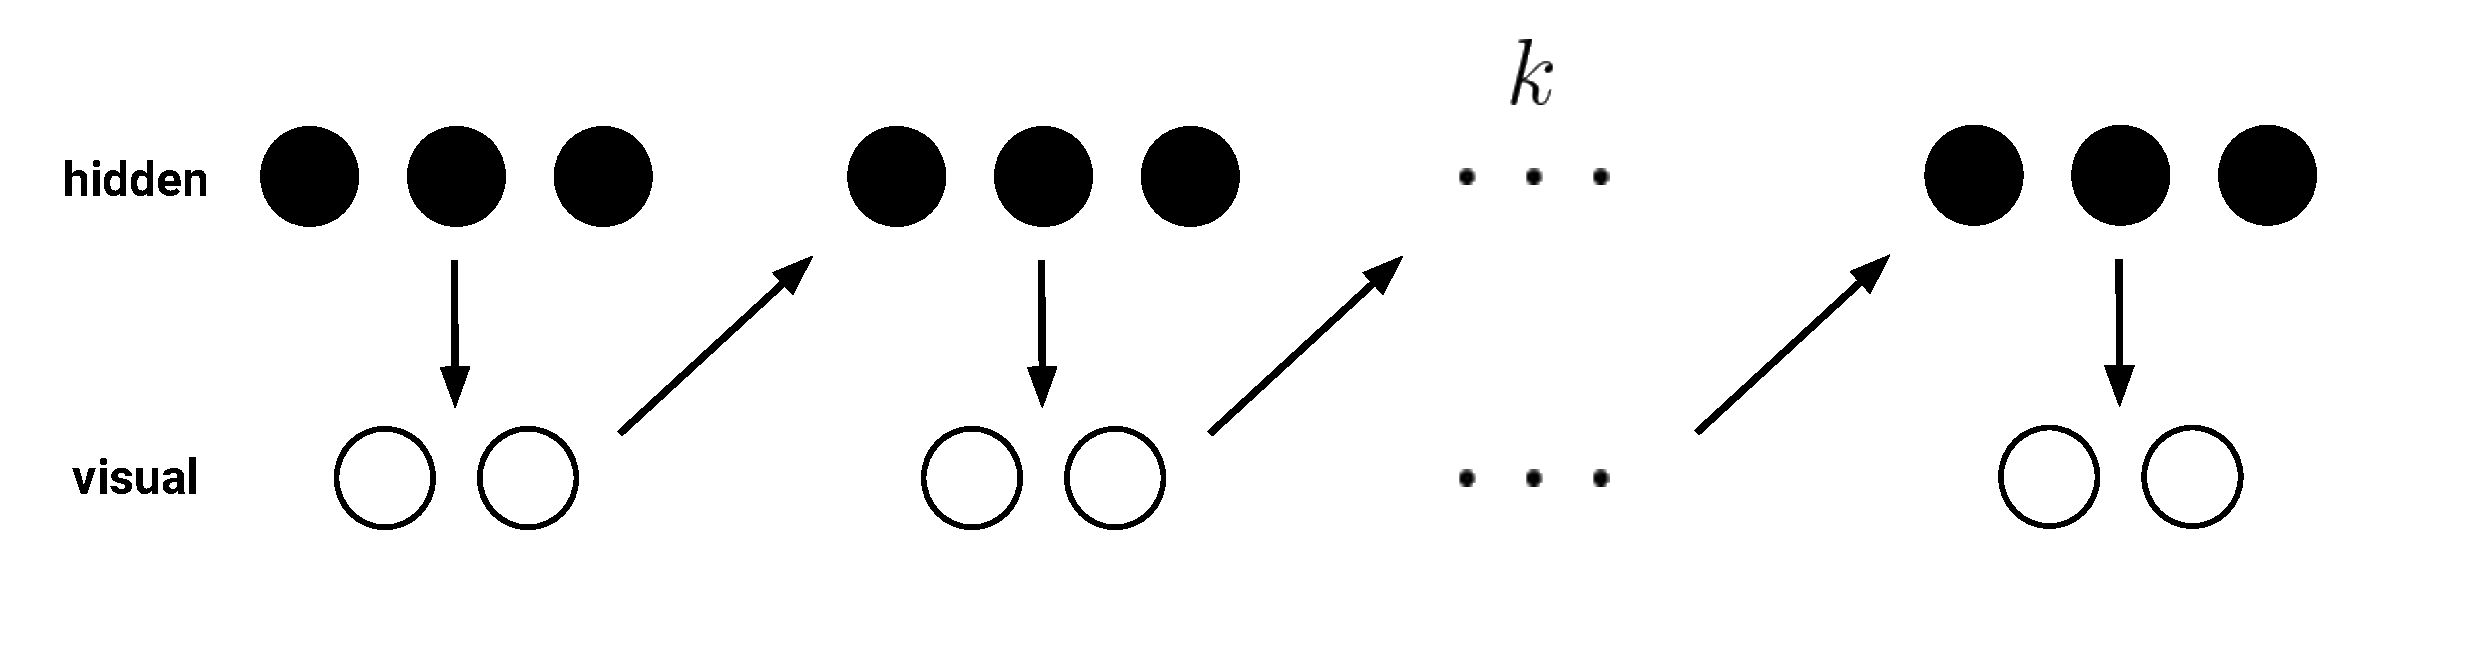
\includegraphics[width=\textwidth]{Figures/Drawn/machinelearning/gibbs_sampling.pdf}
  \end{center}
  \caption{Gibbs sampling done $k$ times. The first hidden layer is generated randomly by a uniform distribution.}
\end{figure}

Sampling of a layer is done by the conditional distributions:

\begin{center}
\begin{gather}
    P(\boldsymbol{v} | \boldsymbol{h} ) = \prod_{i \in \boldsymbol{v}} P(v_i | \boldsymbol{h} ) \\ 
    P(\boldsymbol{h} | \boldsymbol{v} ) = \prod_{j \in \boldsymbol{h}} P(h_j | \boldsymbol{v} ) \; .
\end{gather}
\end{center}
Repeated sampling converges, as shown by Christian P. Robert and George Casella in "Monte Carlo Statistical Methods", \cite{Robert1999} (chapter 10.2.1 page 378).


